\documentclass[10pt,twocolumn]{article}

\usepackage[letterpaper,margin=0.58in,columnsep=0.25in]{geometry}
\usepackage[T1]{fontenc}
\usepackage[utf8]{inputenc}
\usepackage{lmodern}
\usepackage{microtype}
\usepackage{amsmath,amssymb,mathtools}
\usepackage{booktabs}
\usepackage[dvipsnames]{xcolor}
\usepackage{graphicx}
\usepackage{tikz}
\usetikzlibrary{arrows.meta,positioning,calc}
\usepackage{enumitem}
\usepackage{caption}
\usepackage{fancyhdr}
\usepackage[colorlinks=true,linkcolor=MidnightBlue,citecolor=MidnightBlue,urlcolor=MidnightBlue]{hyperref}

\definecolor{ink}{HTML}{253142}
\definecolor{accent}{HTML}{E76623}
\definecolor{soft}{HTML}{EEF1F5}
\definecolor{muted}{HTML}{64748B}
\setlength{\parindent}{0.9em}
\setlength{\parskip}{0.12em}
\setlength{\abovedisplayskip}{5pt plus 2pt minus 2pt}
\setlength{\belowdisplayskip}{5pt plus 2pt minus 2pt}
\setlength{\textfloatsep}{8pt plus 2pt minus 2pt}
\setlength{\floatsep}{7pt plus 2pt minus 2pt}
\setlist{nosep,leftmargin=1.2em}
\captionsetup{font=small,labelfont={bf,color=ink}}
\pagestyle{fancy}
\fancyhf{}
\fancyhead[L]{\footnotesize MPTS Bayesian Profile Lab}
\fancyhead[R]{\footnotesize Pedagogical project companion}
\fancyfoot[C]{\footnotesize\thepage}
\renewcommand{\headrulewidth}{0.3pt}
\renewcommand{\sectionmark}[1]{}
\renewcommand{\thesection}{\arabic{section}}
\renewcommand{\thesubsection}{\thesection.\arabic{subsection}}
\newcommand{\GP}{\mathcal{GP}}
\newcommand{\Normal}{\mathcal{N}}
\newcommand{\Data}{\mathcal{D}}
\newcommand{\R}{\mathbb{R}}
\newcommand{\dd}{\,\mathrm{d}}
\newcommand{\Te}{T_e}
\newcommand{\nelec}{n_e}
\newcommand{\code}[1]{\texttt{#1}}

\title{\vspace{-1.8em}\color{ink}\bfseries\LARGE
From Noisy MPTS Points to Positive Plasma Profiles\\[-0.05em]
\large A Pedagogical Companion to the Bayesian Profile Lab}
\author{UW Plasma Hackathon Project}
\date{24 August 2026}

\begin{document}

\twocolumn[
\maketitle
\vspace{-1.1em}
\begin{minipage}{0.96\textwidth}
\small
\textbf{Technical abstract.}
The bundled NSTX multipoint Thomson-scattering file already contains processed
electron-temperature and electron-density measurements, their reported
standard uncertainties, and the major radius of each spatial channel.  The
project therefore solves a noisy-function reconstruction problem.  For either
physical quantity $f\in\{\Te,\nelec\}$, a dimensionless latent field
$z:I\rightarrow\R$ receives a stationary Mat\'ern-$5/2$ Gaussian-process prior,
the physical profile is constructed as $f(R)=f_{\rm ref}\exp z(R)>0$, and the
reported uncertainty remains an additive Gaussian likelihood in keV or
cm$^{-3}$.  A Laplace approximation at each of nine correlation-length
quadrature nodes supplies an interactive approximation to the non-Gaussian
posterior.  Analytic kernel derivatives produce correlated samples of $z$ and
$z'$, from which the program computes $f'$, $d\log f/dR$, and the reciprocal
scale length.  A sign-identification gate withholds the reciprocal wherever
the posterior supports a zero gradient.  The implementation completed all
1,486 temperature and density fits in the bundled sweep, eliminated the 590
negative-median profiles produced by the original linear-space baseline, and
passed compact synthetic calibration tests.  Its intervals remain conditional
on the stated stationary-kernel and likelihood family, its radial coordinate is
geometric major radius, and its Laplace/quadrature posterior still requires
comparison against full posterior sampling before scientific deployment.
\end{minipage}
\vspace{0.7em}
]

\section{The measurement already exists}

The governing distinction appears before any regression equation.  NSTX-U's
diagnostic analysis converts calibrated optical signals into local estimates
of $\Te$ and $\nelec$.  The hackathon file begins after that conversion.  One
selected shot and acquisition time supplies
\begin{align}
\Data_T&=\{(R_i,T_{e,i},\sigma_{T,i})\}_{i=1}^{N_T},\\
\Data_n&=\{(R_i,n_{e,i},\sigma_{n,i})\}_{i=1}^{N_n}. \label{eq:data}
\end{align}
Here $R_i$ is the geometric machine major radius of channel $i$;
$\sigma_{T,i}$ and $\sigma_{n,i}$ are the standard uncertainties reported by
the processed diagnostic.  The inference target is a pair of positive
functions on the measured interval $I=[R_{\min},R_{\max}]$:
\begin{equation}
(\Te,\nelec)\in C^1(I,\R_{>0})\times C^1(I,\R_{>0}).
\end{equation}
The first derivative is included in the target space because the requested
outputs contain $df/dR$ and a normalized gradient.

The HDF5 reader found 14 shots and 743 acquisition times.  Each acquisition
contains 30 radii and therefore defines two independent profile problems,
giving $2\times743=1{,}486$ fits in the complete sweep.  In the default case,
shot 141687 at $0.3150$ s, the channels span $27.60$--$156.17$ cm with a
median separation of $2.916$ cm.  The median reported relative uncertainties
are $4.94\%$ for temperature and $4.47\%$ for density.

\begin{figure*}[t]
\centering
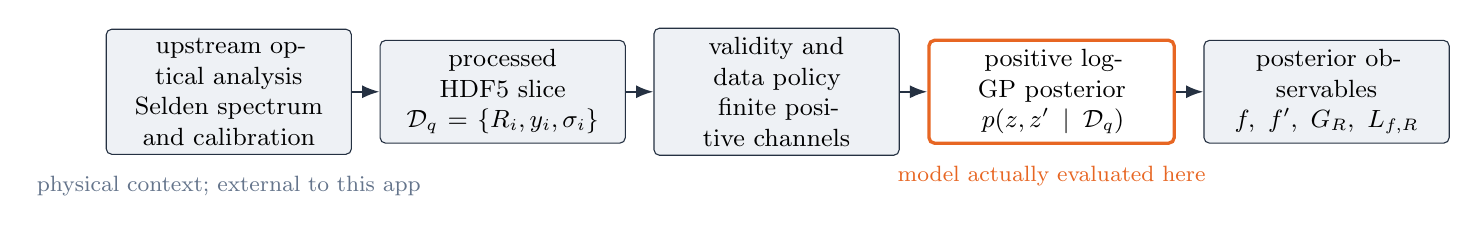
\begin{tikzpicture}[
  node distance=3.5mm,
  every node/.style={font=\small,align=center},
  stage/.style={draw=ink,rounded corners=2pt,fill=soft,minimum height=11mm,text width=2.88cm},
  main/.style={draw=accent,very thick,rounded corners=2pt,fill=white,minimum height=11mm,text width=2.88cm},
  arrow/.style={-{Latex[length=2.2mm]},thick,color=ink}
]
\node[stage] (up) {upstream optical analysis\\Selden spectrum and calibration};
\node[stage,right=of up] (data) {processed HDF5 slice\\$\Data_q=\{R_i,y_i,\sigma_i\}$};
\node[stage,right=of data] (gate) {validity and data policy\\finite positive channels};
\node[main,right=of gate] (post) {positive log-GP posterior\\$p(z,z'\mid\Data_q)$};
\node[stage,right=of post] (out) {posterior observables\\$f,\ f',\ G_R,\ L_{f,R}$};
\draw[arrow] (up)--(data);
\draw[arrow] (data)--(gate);
\draw[arrow] (gate)--(post);
\draw[arrow] (post)--(out);
\node[below=1.5mm of up,font=\footnotesize,color=muted] {physical context; external to this app};
\node[below=1.5mm of post,font=\footnotesize,color=accent] {model actually evaluated here};
\end{tikzpicture}
\caption{The calculation map.  The upstream Thomson-spectrum fit explains the
origin of the measurements; the repository begins with processed profile
points and propagates their uncertainty through a positive spatial model.}
\label{fig:map}
\end{figure*}

Figure~\ref{fig:map} fixes the boundary between plasma-diagnostic physics and
the reconstruction performed here.  The upstream NSTX-U pipeline evaluates a
relativistic Selden spectrum through the measured polychromator response,
adjusts temperature and amplitude by a spectral chi-squared fit, and converts
the calibrated amplitude into density \cite{laggner2019}.  A compact channel
model is
\begin{equation}
\mu_j=b_j+A E_L\nelec\!\int
\mathcal T_j(\lambda)\eta_j(\lambda)
S_{\lambda}^{\rm Selden}(\lambda;\Te,\theta)\dd\lambda .
\label{eq:thomson}
\end{equation}
The expected signal $\mu_j$ in optical channel $j$ combines background $b_j$,
laser energy $E_L$, density $\nelec$, filter transmission $\mathcal T_j$,
detector efficiency $\eta_j$, and the temperature-dependent spectral shape.
Equation~\eqref{eq:thomson} supplies physical provenance.  No variable on its
left-hand side is present in the bundled HDF5 file, so the app does not
evaluate this equation.

\section{A positive function from uncertain points}

Choose one quantity $q\in\{T,n\}$ and write its processed observations as
$y_i$ with standard uncertainties $\sigma_i$.  The measurement model is
heteroscedastic: each channel carries its own noise variance,
\begin{equation}
y_i=f(R_i)+\epsilon_i,qquad
\epsilon_i\sim\Normal(0,\sigma_i^2).
\label{eq:likelihood-linear}
\end{equation}
Consequently, a small-$\sigma_i$ channel contributes greater likelihood
curvature than a large-$\sigma_i$ channel.  The optional relative-uncertainty
filter changes which observations enter the posterior; it is a sensitivity
control, since Equation~\eqref{eq:likelihood-linear} already down-weights a
finite high-uncertainty point.

Temperature and density occupy $\R_{>0}$.  We encode that support through a
latent logarithmic coordinate.  Let $f_{\rm ref}>0$ be a fixed physical scale:
$1$ keV for $\Te$ and $10^{13}$ cm$^{-3}$ for $\nelec$.  Construct
\begin{equation}
\begin{aligned}
z(R)&=\beta+u(R),&
u&\sim\GP(0,k_{5/2}),\\
f(R)&=f_{\rm ref}\exp z(R),&
y_i\mid z&\sim\Normal\!\left(f_{\rm ref}e^{z(R_i)},\sigma_i^2\right).
\end{aligned}
\label{eq:positive-likelihood}
\end{equation}
The latent field $z:I\rightarrow\R$ is dimensionless; exponentiation maps it
into a positive physical profile.  The likelihood in
Equation~\eqref{eq:positive-likelihood} remains Gaussian in the original
measurement units.  Thus positivity of the latent physical state does not
replace the diagnostic's additive error statement with a lognormal observation
model.

The constant $\beta$ sets the log-profile level.  The present priors are
\begin{equation}
\begin{aligned}
\beta&\sim\Normal(0,2^2),&
\sigma_z&\sim\operatorname{HalfNormal}(1),\\
\log(\ell/D)&\sim\Normal(\log0.12,0.75^2).&&
\end{aligned}
\label{eq:priors}
\end{equation}
where $D=R_{\max}-R_{\min}$, $\sigma_z$ is the latent covariance amplitude,
and $\ell$ is its radial correlation length.  The code rescales radius to
$x=(R-R_{\min})/D\in[0,1]$ for computation, then restores physical derivative
units through $d/dR=D^{-1}d/dx$.

\subsection{Smoothness as a scientific prior}

For $d=|R-R'|$ and $a=\sqrt{5}/\ell$, the default covariance is
\begin{equation}
k_{5/2}(R,R')=\sigma_z^2
\left(1+ad+\frac{a^2d^2}{3}\right)e^{-ad}.
\label{eq:matern}
\end{equation}
The correlation length $\ell$ defines the radial scale over which latent
profile values inform one another.  A short $\ell$ admits local structure; a
long $\ell$ couples distant channels into a broad profile.  The Mat\'ern-$5/2$
family supplies a regular first-derivative process while retaining less prior
smoothness than the radial-basis-function kernel.  The implementation also
prevents inferred correlation lengths below the typical channel separation,
because no observation pattern can resolve repeatable sub-channel structure.

The project fits $\Te$ and $\nelec$ independently.  This avoids asserting an
unvalidated cross-quantity covariance.  It also fits each acquisition time
independently, so rapid temporal changes are neither pooled nor smoothed across
frames.

\section{The posterior moves through derivatives}

Because $f=f_{\rm ref}e^z$, Equation~\eqref{eq:positive-likelihood} is
nonlinear in the Gaussian field $z$.  Let
$\mathbf z=(z(R_1),\ldots,z(R_N))^{\mathsf T}$ and
$K_{XX}=[k(R_i,R_j)]_{ij}$.  Apart from constants, the negative log posterior
at fixed hyperparameters is
\begin{align}
\Phi(\mathbf z,\beta,\sigma_z;\ell)
={}&\frac12\sum_{i=1}^{N}
\frac{(y_i-f_{\rm ref}e^{z_i})^2}{\sigma_i^2}
+\frac12\sum_{i=1}^{N}\log\sigma_i^2 \notag\\
&+\frac12(\mathbf z-\beta\mathbf1)^{\mathsf T}
K_{XX}^{-1}(\mathbf z-\beta\mathbf1)\notag\\
&+\frac12\log|K_{XX}|+\Phi_{\rm prior}.
\label{eq:objective}
\end{align}
Here $\Phi_{\rm prior}$ contains Equation~\eqref{eq:priors}.  The optimized
variables $\mathbf z$, $\beta$, and $\sigma_z$ remain inside the posterior
approximation; they have not been replaced by a smoothed curve.

Interactive inference proceeds through a finite mixture:
\begin{enumerate}
\item Place nine quadrature nodes in $\log(\ell/D)$ between the channel-spacing
floor and the prior-supported upper range.
\item At each node $m$, minimize $\Phi$ with L-BFGS-B and compute the local
Hessian $H_m=\nabla^2\Phi(\widehat\vartheta_m)$.
\item Form a stabilized Laplace covariance $H_m^{-1}$ and an evidence weight
\begin{equation}
\log w_m\doteq-\Phi(\widehat\vartheta_m)
-\frac12\log|H_m|+\log p(\log\ell_m)+\log\Delta_m.
\end{equation}
\item Draw latent and hyperparameter points from the normalized mixture, then
draw conditional functions and derivatives on a dense radial grid.
\end{enumerate}
The symbol $\doteq$ marks a Laplace/quadrature approximation.  Integration over
several length scales carries materially more posterior volume information
than one optimized empirical-Bayes length, yet it remains an approximation to
full Bayesian sampling.

\subsection{Analytic differentiation preserves correlation}

For $\delta=R-R'$ and $d=|\delta|$, differentiating
Equation~\eqref{eq:matern} gives
\begin{align}
\operatorname{Cov}[z(R),z'(R')]
&=\frac{\sigma_z^2a^2}{3}\,
\delta(1+ad)e^{-ad},\label{eq:crosscov}\\
\operatorname{Cov}[z'(R),z'(R')]
&=\frac{\sigma_z^2a^2}{3}
\left(1+ad-a^2d^2\right)e^{-ad}.
\label{eq:derivcov}
\end{align}
These are covariances, not finite-difference recipes.  They construct one joint
random object containing profile values and radial derivatives
\cite{solak2003}.  At evaluation radii $\mathbf R_*$, stack
\begin{equation}
\mathbf d_*=\binom{\mathbf z_*}{\mathbf g_*},
\qquad
\mathbf g_*=(z'(R_{*,1}),\ldots,z'(R_{*,M}))^{\mathsf T}.
\end{equation}
Conditional on one posterior draw of the training latent values and kernel
parameters,
\begin{align}
\mathbf d_*\mid\mathbf z_X,\phi
&\sim\Normal(\boldsymbol\mu_d,C_d),\label{eq:jointconditional}\\
\boldsymbol\mu_d
&=\mathbf m_d+K_{dX}K_{XX}^{-1}(\mathbf z_X-\mathbf m_X),\\
C_d&=K_{dd}-K_{dX}K_{XX}^{-1}K_{Xd}.
\end{align}
The off-diagonal blocks retain the dependence between $z$ and $z'$.  Every
derived posterior sample therefore represents one internally consistent
profile and gradient.

\section{One sample, four physical observables}

Let $(z^{(s)},z'^{(s)})$ be sample $s$ from
Equation~\eqref{eq:jointconditional}.  The samplewise map is
\begin{align}
f^{(s)}(R)&=f_{\rm ref}e^{z^{(s)}(R)},\label{eq:sample-profile}\\
f'^{(s)}(R)&=f^{(s)}(R)z'^{(s)}(R),\label{eq:sample-gradient}\\
G_R^{(s)}(R)&=\frac{f'^{(s)}(R)}{f^{(s)}(R)}=z'^{(s)}(R),\label{eq:sample-loggrad}\\
L_{f,R}^{(s)}(R)&=\frac{f^{(s)}(R)}{f'^{(s)}(R)}
=\frac{1}{z'^{(s)}(R)}.\label{eq:sample-scale}
\end{align}
The profile has the physical units of $f$; $f'$ carries those units per cm;
$G_R=d\log f/dR$ has units cm$^{-1}$; and $L_{f,R}$ has units cm.  Pointwise
medians and selected quantiles across $s=1,\ldots,S$ form the displayed central
curves and credible intervals.  They are pointwise posterior bands: at each
radius they contain the selected posterior mass under this model.  They are
not simultaneous whole-function bands or repeated-experiment confidence
guarantees.

The reciprocal in Equation~\eqref{eq:sample-scale} creates a real
identifiability boundary.  At confidence level $c$, define
\begin{equation}
p_+(R)=\Pr[z'(R)>0\mid\Data],\qquad
\alpha=\frac{1-c}{2}.
\end{equation}
The gradient sign is unresolved when
$\alpha<p_+(R)<1-\alpha$.  In that region the posterior crosses the pole at
$z'=0$, so a finite scale length would hide the defining uncertainty.  The app
reports $G_R$ and withholds $L_{f,R}$.  It also withholds the scale length
within two median channel spacings of either measurement boundary, where a
derivative is constrained from only one side.

\begin{figure*}[t]
\centering
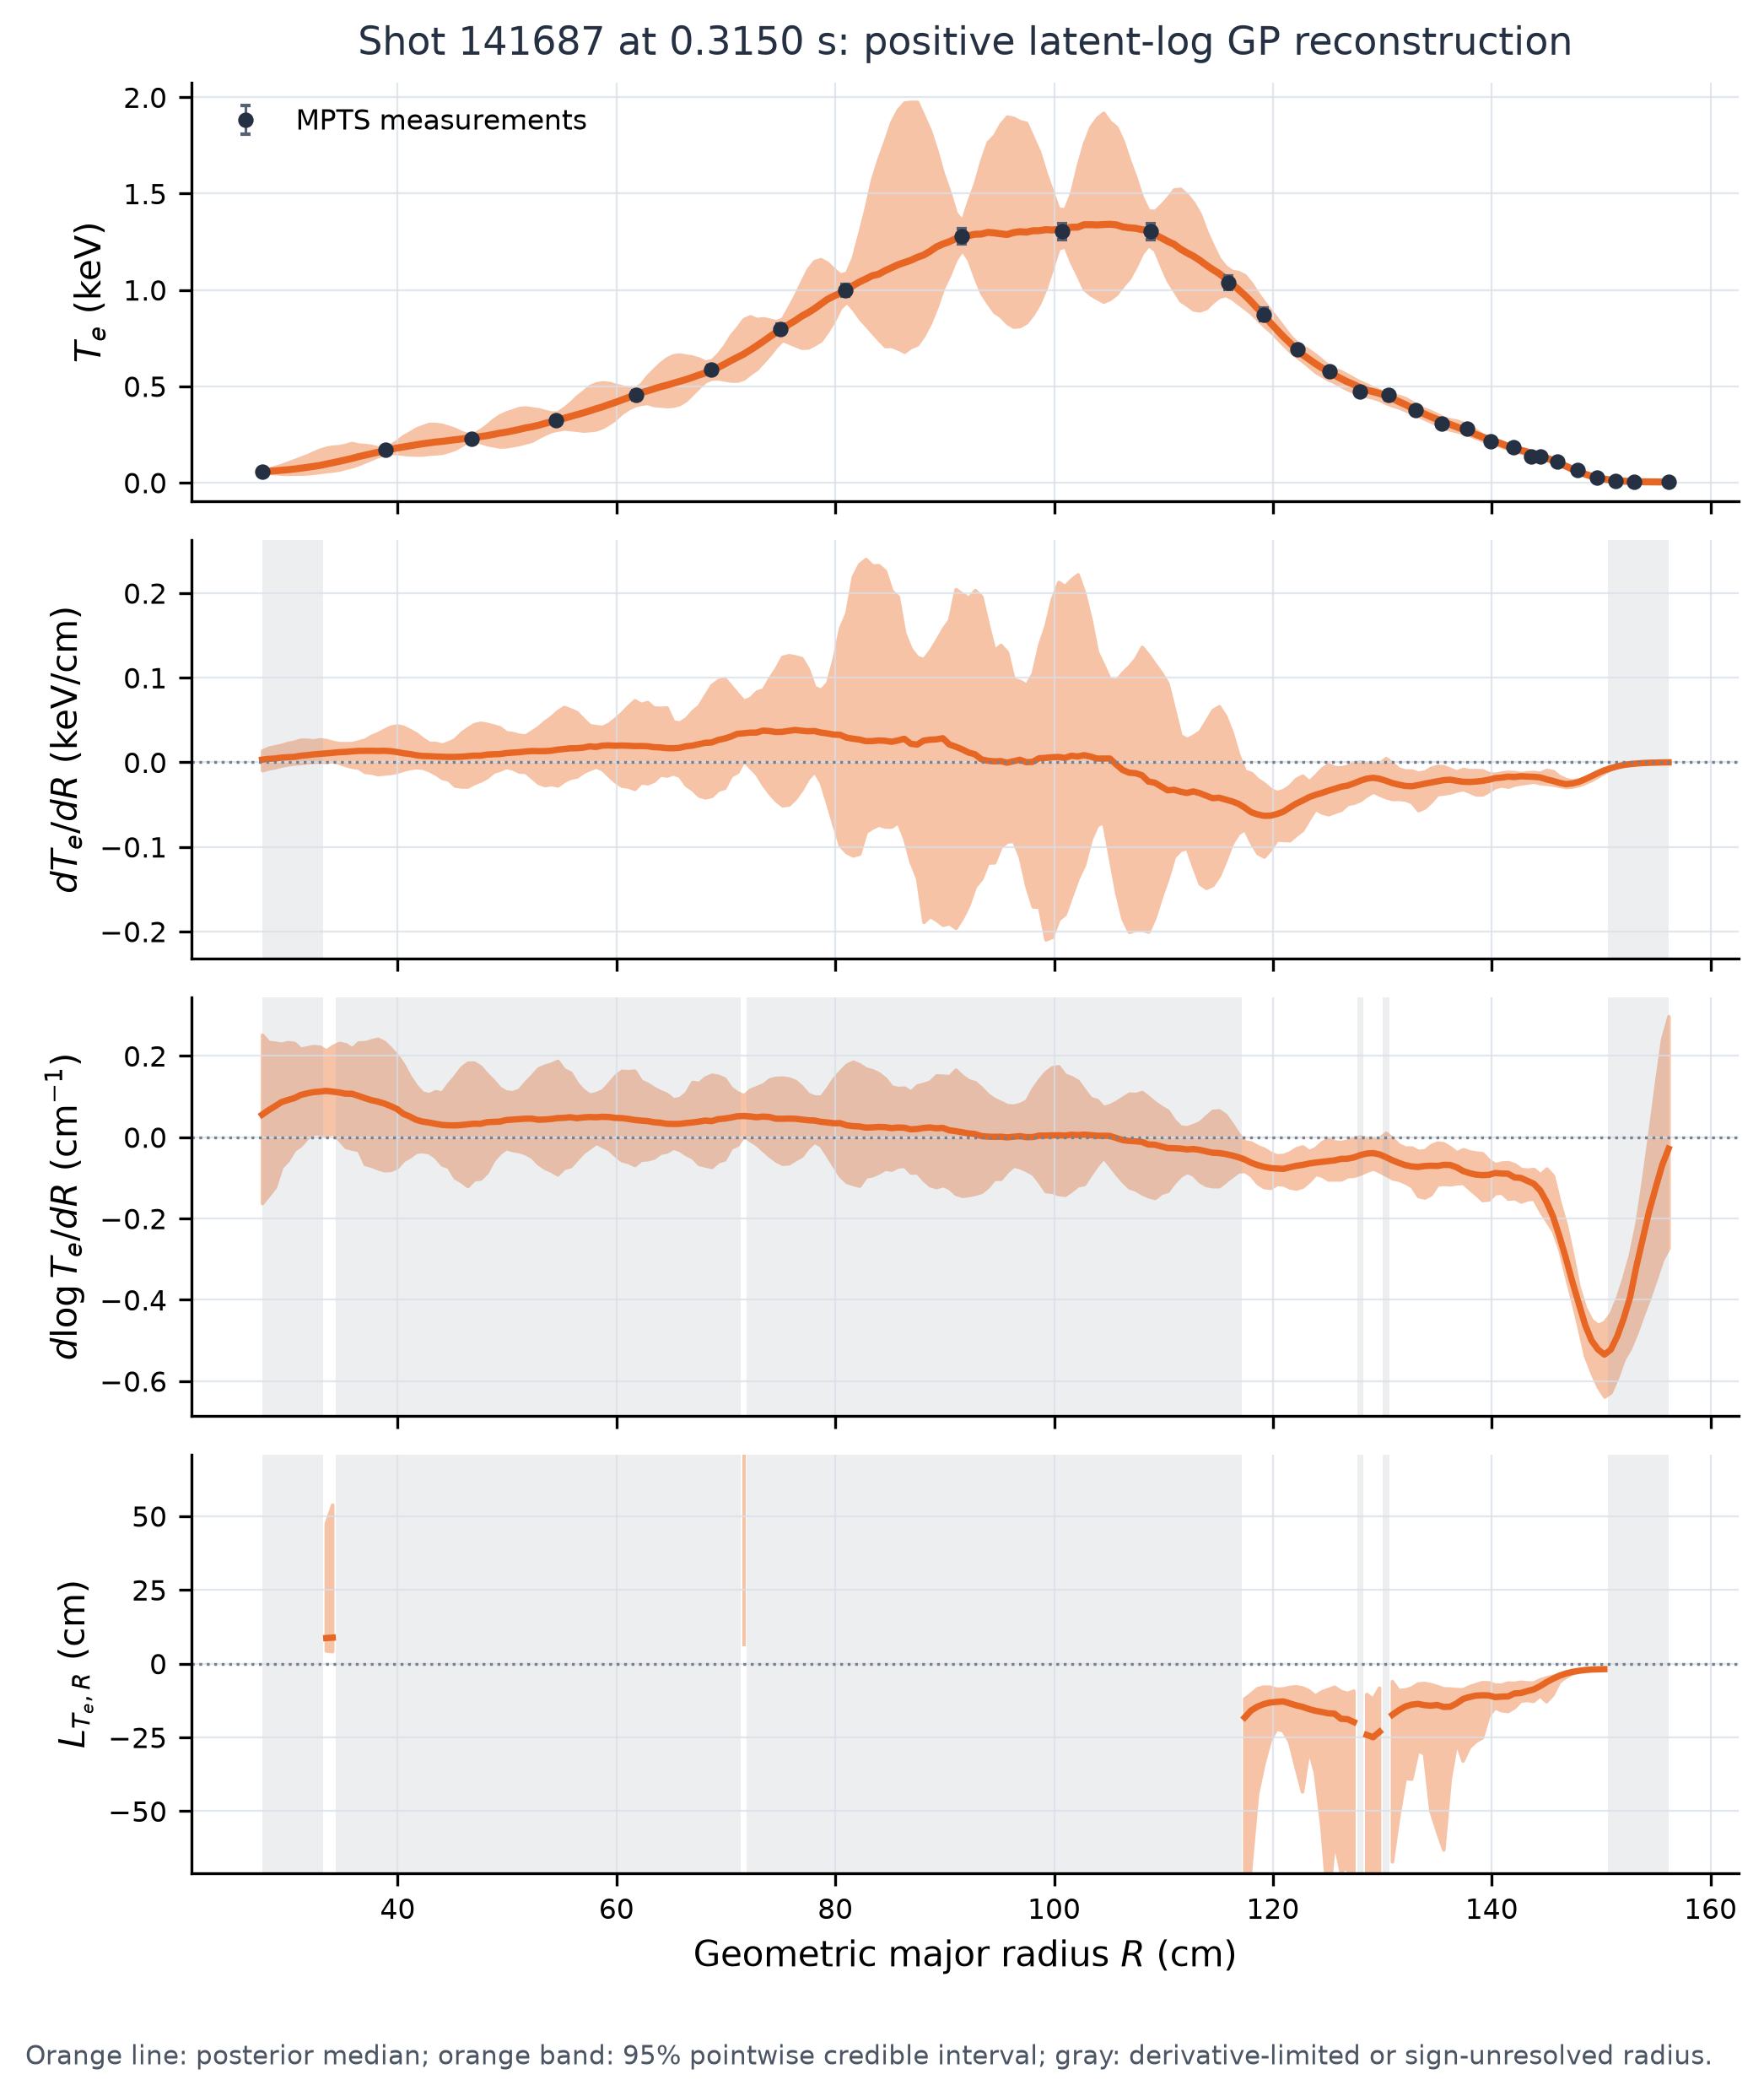
\includegraphics[width=0.78\textwidth]{assets/default_temperature_posterior.png}
\caption{The implemented posterior map for the default temperature case.  The
same correlated samples generate all four panels.  The gray regions mark
one-sided derivative boundaries or radii where the 95\% posterior interval
does not identify the sign of $d\log\Te/dR$; the reciprocal scale length is
therefore omitted.  The broad profile can remain well measured even where its
local derivative is weakly identified.}
\label{fig:defaultfit}
\end{figure*}
\clearpage

Figure~\ref{fig:defaultfit} exposes a central lesson of the project.  Profile
precision does not transfer automatically to derivative precision.  Near a
broad maximum, many positive functions pass through almost the same measured
values while possessing different small slopes.  Their ratio $f/f'$ is the
least stable exactly where the profile appears visually flat.  Refusing to
draw a finite reciprocal in that region is part of the inference, not a
plotting failure.

\section{Major radius is not an outward flux coordinate}

The file supplies geometric major radius $R$.  Along the NSTX-U horizontal
diagnostic chord, increasing $R$ moves toward the magnetic axis on the inboard
branch and away from it on the outboard branch \cite{laggner2019}.  Hence the
sign of $d\log f/dR$ does not encode one globally outward direction.

If an equilibrium reconstruction supplies a flux coordinate $\rho(R)$, then
each monotone branch obeys
\begin{equation}
\frac{d\log f}{d\rho}
=\frac{d\log f/dR}{d\rho/dR}.
\label{eq:fluxmap}
\end{equation}
The denominator changes sign across the magnetic axis.  A transport quantity
such as $a/L_f=-a\,d\log f/dr$ therefore requires an equilibrium map, an outward
minor-radius or flux convention, a normalization length $a$, and propagation
of mapping uncertainty.  The current GUI labels its result
$d\log f/dR$ in cm$^{-1}$ so the coordinate claim remains exact.

\section{Scientific controls, not cosmetic sliders}

Each interface control changes a declared element of the inference or its
reporting policy:
\begin{center}
\small
\setlength{\tabcolsep}{3pt}
\begin{tabular}{p{0.25\columnwidth}p{0.64\columnwidth}}
\toprule
Control & Mathematical role\\
\midrule
Shot, time, quantity & Selects one data set $\Data_q$; $\Te$ and $\nelec$ remain independent.\\
Length scale & Sets or marginalizes the kernel scale $\ell$.\\
Credible level & Sets $c$ and the sign gate $\alpha=(1-c)/2$.\\
Samples & Controls Monte Carlo resolution of transformed quantiles.\\
Edge point & Adds a distinct likelihood term beyond the final measured radius.\\
Relative-error filter & Removes channels for a stated sensitivity analysis.\\
Bottom panel & Displays $G_R$, $p_+$, or the gated reciprocal $L_{f,R}$.\\
\bottomrule
\end{tabular}
\end{center}

No edge condition is active by default.  If independent physics supplies
$R_{\rm edge}>R_{\max}$ and $f_{\rm edge}\pm\sigma_{\rm edge}$, the program
adds
\begin{equation}
y_{\rm edge}\mid z\sim\Normal\!\left(
f_{\rm ref}e^{z(R_{\rm edge})},\sigma_{\rm edge}^2\right).
\end{equation}
Requiring a distinct coordinate prevents a duplicate observation at the last
channel from being mislabeled as a boundary condition.

The provisional validity gate first collects finite positive pairs
$(y_i,\sigma_i)$.  It then computes
\begin{equation}
m_{\rm rel}=\operatorname{median}_i\frac{\sigma_i}{y_i},
\qquad
N_2=\#\{i:y_i/\sigma_i>2\}.
\end{equation}
The profile is labeled unusable when $m_{\rm rel}>1$ or $N_2<6$, cautionary
when $m_{\rm rel}>0.5$ or $N_2<10$, and usable otherwise.  These thresholds
separate obvious absent-signal acquisitions in the hackathon file.  The HDF5
schema lacks upstream saturation and analysis-status flags, so the labels are
a transparent provisional policy rather than a calibrated diagnostic-quality
classifier.

\section{The model changed when the evidence demanded it}

The first implementation used a linear-space heteroscedastic GP.  Its
likelihood honored the supplied uncertainties and its sampled functions could
be differentiated, yet the latent state occupied all of $\R$.  The complete
data sweep located the practical consequence: 590 of 1,486 fits had a negative
posterior median somewhere in the measured interval.  Temperature and density
are positive fields, so this was a support mismatch rather than an occasional
tail event.

The positive map in Equation~\eqref{eq:positive-likelihood} repaired that
specific defect without changing the additive measurement semantics.  The
same sweep then completed every profile with no negative posterior median or
lower band.  Figure~\ref{fig:robustness} records the numerical diagnostic that
forced the model decision.

\begin{figure}[t]
\centering
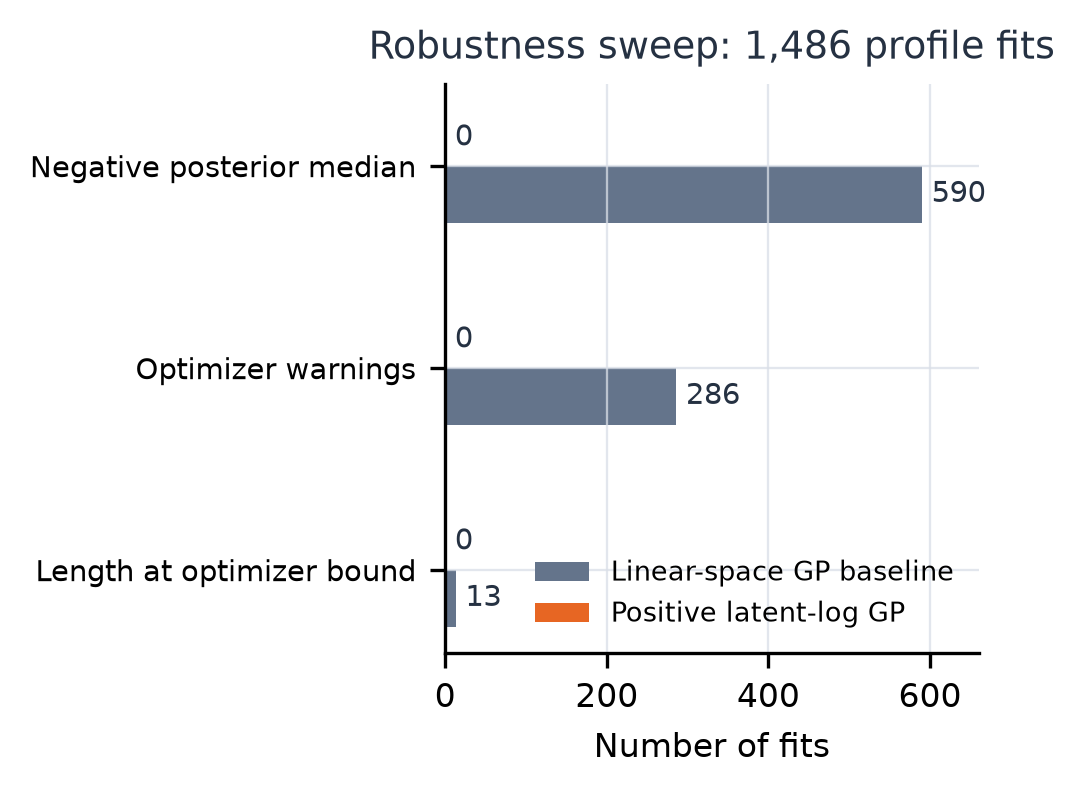
\includegraphics[width=\columnwidth]{assets/model_robustness_comparison.png}
\caption{Numerical failure indicators from the bundled-profile sweeps.  The
positive latent-log model removes negative physical support by construction
and did not trigger the optimizer-warning or boundary counters used in this
compact sweep.  The two sweeps used their respective hackathon inference
implementations; the bars diagnose failure modes, not equal-cost runtime.}
\label{fig:robustness}
\end{figure}

The repair also changed what the app is willing to report.  Under the positive
model, 675 profiles had more than 90\% of their radial scale length withheld;
the plug-in linear baseline produced 170.  The larger count follows the
posterior sign gate, hyperparameter mixture, and endpoint exclusion.  It
expresses weaker evidence for a reciprocal gradient even when the underlying
profile fit succeeds.

Synthetic functions provide a separate check because their exact derivatives
are known.  Twenty independent noise realizations were fitted for positive
linear, peaked, and flat truths at 25 measurement locations.  The table reports
the fraction of evaluation radii at which a nominal 95\% pointwise band
contained the truth, averaged across repetitions.

\begin{center}
\small
\begin{tabular}{lrrr}
\toprule
Truth & $f$ & reportable $f'$ & reportable $G_R$\\
\midrule
Linear & 91.3\% & 93.8\% & 94.3\%\\
Peaked & 94.1\% & 96.3\% & 96.2\%\\
Flat & 95.2\% & 100.0\% & 100.0\%\\
\bottomrule
\end{tabular}
\end{center}

The flat truth gives the most important falsification: its inferred gradient
interval contained zero over the entire grid, and the scale length was
withheld everywhere.  All synthetic positive-profile lower bands remained
positive.  Twenty repetitions are adequate for a compact implementation test;
they do not estimate 95\% coverage to production precision.

\section{The application as an executable argument}

The repository keeps the scientific maps in small modules.  Their composition
is
\begin{equation}
\begin{aligned}
\code{data.py}&\longrightarrow
\code{gp.py}/\code{positive\_gp.py}\\
&\longrightarrow\code{plotting.py}
\longrightarrow\code{app.py}.
\end{aligned}
\end{equation}
\code{data.py} preserves the HDF5 $(R,\text{time})$ axes and units.
\code{gp.py} defines the shared configuration, validity gate, result object,
and labeled linear baseline.  \code{positive\_gp.py} evaluates
Equations~\eqref{eq:objective}--\eqref{eq:jointconditional}, draws the mixture,
and performs Equations~\eqref{eq:sample-profile}--\eqref{eq:sample-scale}.
\code{plotting.py} converts one posterior summary into aligned profile,
gradient, and derived panels.  \code{app.py} binds those maps to the shot,
time, quantity, prior, boundary, and posterior controls.

Unit tests check the schema, ordered credible bands, derivative units, flat
profile withholding, positive support, validity classification, distinct edge
coordinates, optional data filtering, and the presence of multiple
Laplace/quadrature components.  The synthetic and all-profile validation
scripts exercise a different axis: whether the assembled program behaves
sensibly on known functions and on every supplied acquisition.

\section{What has been established}

The project constructs a coherent Bayesian path from processed MPTS points to
positive spatial profiles and correlated gradient uncertainty.  The
heteroscedastic likelihood preserves each supplied error bar; the log latent
field enforces the physical support; the Mat\'ern covariance defines radial
regularity; analytic differentiation carries the same posterior into $f'$ and
$d\log f/dR$; and the sign gate refuses to replace an unresolved zero
denominator with a visually convenient scale length.  The GUI exposes these
choices as scientific controls and preserves geometric major radius in every
label.

The present evidence supports a hackathon reconstruction tool and an
exploratory scientific workflow.  Four extensions separate it from a validated
diagnostic product:
\begin{enumerate}
\item compare the Laplace/quadrature mixture with HMC or NUTS on strong, flat,
outlier-contaminated, and absent-signal cases;
\item ingest upstream channel validity, saturation, over-range, and under-range
status rather than relying on the provisional profile gate;
\item perform leave-one-channel-out and radial-block posterior predictive
checks before adding a robust mixture likelihood; and
\item propagate an equilibrium ensemble before converting $R$ derivatives into
outward flux-surface gradients or $a/L_f$.
\end{enumerate}
These are distinct validity axes.  Successful optimization establishes
numerical completion; positive support establishes one physical constraint;
synthetic coverage probes interval calibration; and equilibrium mapping is
required for transport interpretation.  No one axis certifies the others.

\section*{Oral reconstruction}

\begin{enumerate}
\item Starting from one HDF5 slice, reconstruct the complete map to a displayed
$L_{f,R}$ sample and identify where measurement uncertainty enters.
\item Explain why $f=f_{\rm ref}e^z$ enforces positivity without imposing a
lognormal likelihood on the processed measurements.
\item Derive $f'=fz'$ and use it to explain why $d\log f/dR$ is the primary
normalized-gradient output.
\item State the posterior event that makes a finite $L_{f,R}$ scientifically
unreportable, then distinguish it from endpoint derivative limitation.
\item Identify which evidence supports numerical completion, positive support,
synthetic calibration, and flux-coordinate interpretation.
\end{enumerate}

\begin{thebibliography}{9}
\footnotesize
\setlength{\itemsep}{1pt}
\setlength{\parsep}{0pt}

\bibitem{laggner2019}
F. M. Laggner et al., ``A scalable real-time framework for Thomson scattering
analysis: Application to NSTX-U,'' \emph{Review of Scientific Instruments}
\textbf{90}, 043501 (2019).
\href{https://doi.org/10.1063/1.5088248}{doi:10.1063/1.5088248}.

\bibitem{chilenski2015}
M. A. Chilenski et al., ``Improved profile fitting and quantification of
uncertainty in experimental measurements of impurity transport coefficients
using Gaussian process regression,'' \emph{Nuclear Fusion} \textbf{55},
023012 (2015).
\href{https://doi.org/10.1088/0029-5515/55/2/023012}{doi:10.1088/0029-5515/55/2/023012}.

\bibitem{kwak2020}
S. Kwak et al., ``Bayesian modelling of Thomson scattering and multichannel
interferometer diagnostics using Gaussian processes,'' \emph{Nuclear Fusion}
\textbf{60}, 046009 (2020).
\href{https://doi.org/10.1088/1741-4326/ab686e}{doi:10.1088/1741-4326/ab686e}.

\bibitem{solak2003}
E. Solak et al.,
``Derivative observations in Gaussian process models of dynamic systems,''
\emph{Advances in Neural Information Processing Systems} \textbf{15} (2003).
\href{https://papers.nips.cc/paper/2287-derivative-observations-in-gaussian-process-models-of-dynamic-systems}{papers.nips.cc/paper/2287}.

\bibitem{rasmussen2006}
C. E. Rasmussen and C. K. I. Williams, \emph{Gaussian Processes for Machine
Learning}, MIT Press (2006).
\href{https://gaussianprocess.org/gpml/}{gaussianprocess.org/gpml}.

\end{thebibliography}

\end{document}
